\chapter{System Design}

To design a game we are faced with a lot of design choices. To make the right choice can determine how the finished result will be met by the audience. We will in this chapter look into which design choices we have made to have a general idea about how our game will be designed.


\section{Infinite World}

As our world will keep on generating infinitely we will need some way of handle the world loading. As most computers have a limited amount of memory we cannot keep generating new content without also taking care of removing the old content. The way most other games handle this problem is to divide the world into chunks of a desirable size.

Chunks are used in numerous ways, for instance as explain in\cite{Chucks} chunks can be used to divide 3D meshes of a terrain into smaller areas to increase the detail level of the terrain. We can adapt on this idea to create infinite world, as we can make a bunch of smaller terrains that linked together would look like a single huge terrain. As seen in Table \ref{table1} we illustrate a terrain divided into 9 chunks with the player standing in the middle at position 0;0.

\begin{table}[H]
	\begin{center}
		\begin{tabular}{ | M{30pt} | M{30pt} | M{30pt} |N}
			\hline
			 -1;1 & 0;1 & 1;1 & \\[30pt] \hline
			-1;0 & \cellcolor{lightgray}0;0 & 1;0 & \\[30pt] \hline
			-1;-1 & 0;-1 & 1;-1 & \\[30pt] \hline
		\end{tabular}
	\end{center}
\caption{The table illustrate a division of a terrain into 9 chunks with the player in the highlighted center chunk.}
\label{table1}
\end{table}

As the player moves around we will need to create more content for the player to explorer, but also to remove old content so that the game does not use too much of the host computer's memory. When ever the player move to either the top-, bottom-, right-, or leftmost chunks a new column or row of chunks will be generated, but the column or row of chucks at the opposite side will also be removed.

We illustrate this process in Table \ref{table2} where the player moves from the chunk at 0;0 to 1;0. The game will then generate and add a new column of chunk on the rightmost side, highlighted with green, and then save any changes made to the leftmost column, highlighted with red, and then removes them.

\begin{table}[H]
	\begin{center}
		\begin{tabular}{ | >{\columncolor[rgb]{1.0,0.1,0.1}} M{30pt} | M{30pt} | M{30pt} | >{\columncolor[rgb]{0.1,1.0,0.1}} M{30pt} |N}
			\hline
			
			-1;1 & 0;1 & 1;1 & 2;1 & \\[30pt] \hline
			-1;0 & \cellcolor[rgb]{0.5,0.5,0.5}0;0 & \cellcolor{lightgray}1;0 & 2;0 & \\[30pt] \hline
			-1;-1 & 0;-1 & 1;-1 & 2;-1 & \\[30pt] \hline
		\end{tabular}
	\end{center}
\caption{The table illustrate the transition from one chunk to another, in this table from 0;0 to 1;0, and the new columns of chunks, highlighted with green, being added on the right side, and the column of old chunks, highlighted with red, being saved removed, as the player moves.}
\label{table2}
\end{table}

After this process we have a new column of chunks as the player have moved onto another chunk as seen in Table \ref{table3}, and the process illustrated in Table \ref{table2} recur when a player moves onto any of the outermost chunk.

\begin{table}[H]
	\begin{center}
		\begin{tabular}{ | M{30pt} | M{30pt} | M{30pt} |N}
			\hline
			0;1 & 1;1 & 2;1 & \\[30pt] \hline
			0;0 & \cellcolor{lightgray}1;0 & 2;0 & \\[30pt] \hline
			0;-1 & 1;-1 & 2;-1 & \\[30pt] \hline
		\end{tabular}
	\end{center}
\caption{The table illustrate which chunks is loaded after the player have entered the chunk at 1;0.}
\label{table3}
\end{table}

We have now demonstrated the usage of a basic chunk loader, however with only 9 chunks a problem is introduced, this being that if a player constantly goes back and forth between 2 chunks the process shown in Table \ref{table2} will happen, and the reverse of the process, which mean that the computer will need to regenerate the chunks that was just removed. To solve this we will increase the number of chunks loaded to minimum either 16 (4x4) or 25 (5x5) as this will create a buffer of chunks that is loaded. As seen in Table \ref{table4} the player now have a 3x3 area to move around on at anytime before entering chunks (highlighted with a cyan color) that triggers new chunks to be generated.

\begin{table}[H]
	\begin{center}
		\begin{tabular}{ | >{\columncolor[rgb]{0.80,1,1}} M{30pt} | M{30pt} | M{30pt} | M{30pt} | >{\columncolor[rgb]{0.80,1,1}} M{30pt} |N}
			\hline
			
			-2;2 & \cellcolor[rgb]{0.80,1,1} -1;2 & \cellcolor[rgb]{0.80,1,1} 0;2 & \cellcolor[rgb]{0.80,1,1} 1;2 & 2;2 & \\[30pt]\hline
			-2;1 & -1;1 & 0;1 & 1;1 & 2;1 & \\[30pt] \hline
			-2;0 & -1;0 & \cellcolor{lightgray}0;0 & 1;0 & 2;0 & \\[30pt] \hline
			-2;-1 & -1;-1 & 0;-1 & 1;-1 & 2;-1 & \\[30pt] \hline
			
			-2;-2 & \cellcolor[rgb]{0.80,1,1} -1;-2 & \cellcolor[rgb]{0.80,1,1} 0;-2 & \cellcolor[rgb]{0.80,1,1} 1;-2 & 2;-2 & \\[30pt]\hline
		\end{tabular}
	\end{center}
\caption{The table illustrate a terrain with 25 chunks with the outer most chunk (highlighted with cyan) being the chunks that triggers new chunks to be loaded.}
\label{table4}
\end{table}

It is possible to increase the loaded area, as well as the number of new chunks to add and remove, however it is on the cost of more memory usage. For instance, we could have a 9x9 grid with 81 chunks loaded at once and have the 2 outermost columns be triggers, but this way we do have over 3 times as many chunks as we would in a 5x5 grid and there by also over 3 times as much memory usage. We could make each chunk smaller to reduce the memory usage, but this would require more chunks to be loaded at once for the player to the best view distance.


\section{World Generation}

As we have the terrain divided into chunks we ultimately only need to generate the world per chunk, this meaning we can work with one chunk at a time. To generate the terrain for each chunk we will use noise maps, however as we want smooth transition between the chunks we also need the noise to be smooth and for this we will need to use coherent-noise. The difference between normal noise and coherent-noise is illustrated in \figref{fig:noise}.

Libnoise already implements coherent-noise function in their noise generators, which give it the properties to always return the same output value, when ever the input value is the same. Besides that a coherent-noise function will produce a small change in the output value, if a small change in the input value have been made, and a large change in the output valve if the a large change have been made to the input value\cite{coherentnoise}.

\begin{figure}[H]
		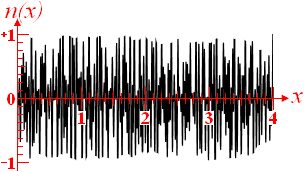
\includegraphics[width=0.49\linewidth]{img/noise}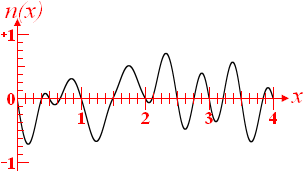
\includegraphics[width=0.49\linewidth]{img/coherentnoise}
		\centering
		\caption{The figure illustrates the difference between noise and coherent-noise in a one-dimensional space. The leftmost is normal noise, where the rightmost is coherent-noise.}
		\label{fig:noise}
\end{figure}

As illustrated in \figref{fig:noise} the non-coherent-noise would result in a very uneven and rough terrain which would ultimately be unplayable. We could smooth the noise before applying it to the terrain, but since coherent-noise do that for us we can simply use that instead. If we look at the rightmost graph in \figref{fig:noise} we can see the $n(x)$ axis represent the output value and the $x$ axis the input value.

If we want to use the rightmost noise to generate terrain, we first need to know the size of the terrain. For simplicity lets say the terrain size is 1. For the first terrain we will use the noise between 0 and 1 which will then result in a huge valley and then a small hill. We then move on to the next terrain, which will be given an offset of 1 as this is the second terrain. This will result in the second will have the noise between 1 and 2 which will result in a valley followed by a hill. This process continues, so the third terrain will have an offset of 2 and have the noise between 2 and 3 and so on.


%\section{World Events}